\documentclass[12pt, oneside]{article} 
\usepackage{amsmath, amsthm, amssymb, calrsfs, wasysym, verbatim, bbm, color, graphics, geometry}
\usepackage{graphicx}
\usepackage{tikz}
\usepackage{amsmath}
\usepackage{graphicx}
\usepackage{amsmath, amssymb, amsthm}
\usepackage{setspace}
\renewcommand{\baselinestretch}{1.5}
\geometry{tmargin=.75in, bmargin=.75in, lmargin=.75in, rmargin = .75in}  

\newcommand{\R}{\mathbb{R}}
\newcommand{\C}{\mathbb{C}}
\newcommand{\Z}{\mathbb{Z}}
\newcommand{\N}{\mathbb{N}}
\newcommand{\Q}{\mathbb{Q}}
\newcommand{\Cdot}{\boldsymbol{\cdot}}

\newtheorem{thm}{Theorem}
\newtheorem{defn}{Definition}
\newtheorem{conv}{Convention}
\newtheorem{rem}{Remark}
\newtheorem{lem}{Lemma}
\newtheorem{cor}{Corollary}


\title{Game Theory}
\author{Kirby CHEN}
\date{Academic Year 2024-2025}

\begin{document}

\maketitle
\tableofcontents

\vspace{.25in}

\section{Nash Equilibrium in Pure Actions}

A game is triple (I,(A$_i$), (u$_i$)) where:
\begin{itemize}
    \item I is a set of players
    \item A$_i$ is the set of actions available to player i
    \item u$_i$ is the payoff function for player i
\end{itemize}

For the moment, the functions \( u_i \) represent ordinal preferences over \( \prod_{i \in I} A_i \).

Note that we are allowing arbitrary externalities.

Consider a game with \( N \) players. A strategy profile  
\[
\mathbf{s^*} = (s_1^*, s_2^*, \dots, s_N^*)
\]  
is a \textbf{Nash equilibrium} of the game if, for every player \( i \),

\[
u_i(s_i^*, \mathbf{s}_{-i}^*) \geq u_i(s_i', \mathbf{s}_{-i}^*)
\]

Given a game \( (I, (A_i)_{i \in I}, (u_i)_{i \in I}) \), a \underline{Nash equilibrium} of this game is an \( n \)-tuple of actions \( (a^*_i)_{i \in I} \) such that for every player \( i \in I \) and for every action \( a_i \in A_i \):

\[
u_i(a^*) \geq u_i(a_i, a^*_{-i}),
\]

where \( (a_i, a^*_{-i}) \) is the list of actions that is identical to \( a^* \) except that we have replaced \( a^*_i \) by \( a_i \).

\underline{\textbf{Interpretation:}} A Nash equilibrium represents a rest point of a learning process in which each player chooses the optimal action assuming that all other players choose the same actions as in the previous period.

\underline{\textbf{Best Response}}: A strategy \( s_i \) is a best response to a strategy profile \( s_{-i} \) if it maximizes the payoff of player i given the strategies of the other players.
\[
u_i(s_i, \mathbf{s}_{-i}) \geq u_i(s_i', \mathbf{s}_{-i})
\]

\underline{\textbf{Best Response Correspondence}}: The best response correspondence of player i is the correspondence that assigns to each strategy profile \( s_{-i} \) the set of best responses of player i to \( s_{-i} \).

\subsection{Key points}
\underline{\textbf{1. Nash equilibria are fixed points of the best reply correspondence.}}

For every player \( i \in I \) define a \underline{best reply correspondence} \( BR_i : \prod_{i \in I} A_i \rightrightarrows A_i \) by setting for every \( a \in \prod_{i \in I} A_i \):

\[
BR_i(a) = \{ a_i \in A_i \mid u_i(a_i, a_{-i}) \geq u_i(a'_i, a_{-i}) \text{ for every } a'_i \in A_i \}.
\]

The \underline{best reply correspondence} \( BR : \prod_{i \in I} A_i \rightrightarrows \prod_{i \in I} A_i \) is defined by setting for every \( a \in \prod_{i \in I} A_i \):

\[
BR(a) = \prod_{i \in I} BR_i(a).
\]

By definition: \( a^* \) is a Nash equilibrium if and only if \( a^* \in BR(a^*) \), i.e., if and only if \( a^* \) is a fixed point of \( BR \).



    \section{Static Games}

\subsection{Case 1: Betrend Competition}
In betrend competition, firm face a total cost curve for producing their goods and simply choose the price for their respective goods. 
Whichever firm has the lower price will get all the customers and if the prices are the same, the customers will be split evenly.
We will assume that identical firms face a constant marginal cost c. The firms simultaneously choose their prices, p1 and p2.
let's look at it from firm 1's perspective (it will be the same for firm firm 2). 

\textbf{Firm 1 has three strategies:}

\begin{itemize}
    \item $p_1 < p_2$: Firm 1 gets all the customers and makes a profit of $p_1 - c$.
    \item $p_1 = p_2$: Firm 1 gets half the customers and makes a profit of $\frac{p_1 - c}{2}$.
    \item $p_1 > p_2$: Firm 1 gets no customers and makes a profit of 0.
\end{itemize}

Naturally, depending on what firm 2's price is, we could have any of these situations. Let s look at some different conditions.

\begin{itemize}
    \item Starting with one extreme, suppose $p_2 > p^m$, the monopoly price.
    \begin{itemize}
        \item If firm 1 chose a price above this, firm 2 would get all of the consumers since their price is lower.
        \item If firm 1 matched this price, they would get half of the consumers.
        \item If firm 1 set a price lower than this, they would get all of the consumers.
    \end{itemize}
    \item Naturally, firm 1 would actually want to set $p_1 = p^m$ in this case since that’s the price that maximizes their profit level.
\end{itemize}

\begin{itemize}
    \item Now, let’s suppose firm 2 chose some price that was at most the monopoly price, i.e., $p_2 \leq p^m$. The same results hold.
    \begin{itemize}
        \item If firm 1 chose a price above this, firm 2 would get all of the consumers since their price is lower.
        \item If firm 1 matched this price, they would get half of the consumers.
        \item If firm 1 set a price lower than this, they would get all of the consumers.
    \end{itemize}
    \item It should be obvious that firm 1 wants to set a price lower than firm 2, $p_1 < p_2$. In fact, to maximize profit, firm 1 wants to undercut firm 2 by as little as possible (a single penny). $p_1 = p_2 - \varepsilon$ where $\varepsilon > 0$ is the smallest possible number that firm 1 can pick.
    \begin{itemize}
        \item That way they get all of the customers while lowering their profit margin by as little as possible.
    \end{itemize}
\end{itemize}

\begin{itemize}
    \item Lastly, suppose firm 2’s price were at or below marginal cost, $p_2 \leq c$.
    \begin{itemize}
        \item If firm 1 chose a price above this, firm 2 would get all of the consumers since their price is lower.
        \item If firm 1 matched this price, they would get half of the consumers.
        \item If firm 1 set a price lower than this, they would get all of the consumers.
    \end{itemize}
    \item Pricing below marginal cost would not be an optimal strategy for firm 1. If $p_1 < c$, firm 1 would actually lose money on each unit sold.
    \begin{itemize}
        \item Thus, the lowest (and only possible) price firm 1 is willing to charge is $p_1 = c$.
    \end{itemize}
\end{itemize}

\begin{itemize}
    \item The analysis for firm 2 is identical.
    \begin{itemize}
        \item If firm 1 prices above the monopoly price, $p_2 = p^m$.
        \item If firm 1 prices between marginal cost and the monopoly price, $p_2 = p_1 - \varepsilon$, where $\varepsilon > 0$ is the smallest possible number greater than zero.
        \item If firm 1 prices at or below marginal cost, $p_2 = c$.
    \end{itemize}
\end{itemize}

\begin{itemize}
    \item Returning to our Nash equilibrium solution concept, we know that our equilibrium is when neither firm has any incentive to deviate from their chosen strategy.
    \begin{itemize}
        \item This occurs where the best response functions intersect.
    \end{itemize}
    \item There is exactly one intersection point in the previous figure, where $p_1 = p_2 = c$. Thus, both firms price at marginal cost in equilibrium.
    \begin{itemize}
        \item This should make sense. Each firm wants to undercut the other to claim the whole market. Yet they can’t undercut anymore once the price is at marginal cost or they’ll suffer losses.
        \item Bertrand competition implies that with just two firms, we reach the perfectly competitive equilibrium.
    \end{itemize}
    \item Since price is set at marginal cost for both firms, economic profit under Bertrand competition equals zero.
\end{itemize}

\begin{figure}[h!]
    \centering
    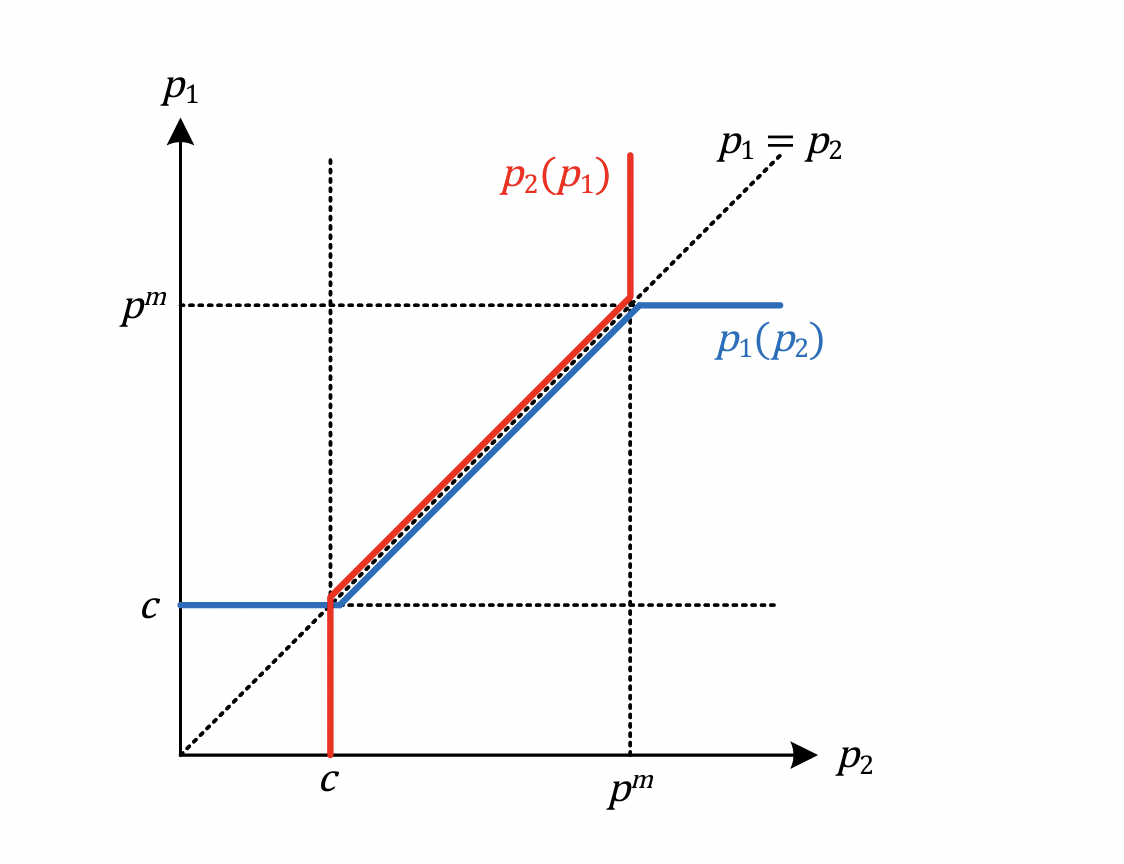
\includegraphics[width=0.8\textwidth]{Figure/Betrend.png} % 图片文件路径
    \caption{EQ} 
    \label{fig:1} 
\end{figure}

\subsection{Case 2: Cournet Competition}

\subsection{Case 3: Stackelberg Competition}

\section{Topic 2: Nash Equilibria in Mixed Actions}

% \subsection{Exponential Distribution}

% \subsection{Poisson Distribution}

% \begin{itemize}

% \item Newtonian mechanics (i.e., ${\bf F} = m{\bf a}$) is an excellent theory; it applies to the vast majority of human-scale (and even interplanetary-scale) physics. 

% \item Apart from relativistic effects at very high velocities (special relativity) or in very strong gravitational fields (general relativity), Newtonian mechanics accurately describes a huge range of phenomena, but around the end of the Nineteenth Century people became aware of some physical effects for which there is no sensible Newtonian explanation.

% \item Examples include:
% \begin{itemize}
% \item the {\bf double slit experiment} (done with light by Thomas Young in 1801, and with electrons by Tonomura in 1986)
% \item the photoelectric effect (analyzed by Einstein in 1905 --- in fact his Nobel-winning work)
% \item the ``quantum Venn diagram'' puzzle, involving the overlaps of three polarizing filters
% \item the stability of the hydrogen atom (i.e., the fact that the electron doesn't lose energy and spiral inward toward the proton).
% \end{itemize}

% \begin{rem}
% How now, brown cow?
% \end{rem}

% \begin{defn}
% The {\em Feynman kernel} is given by
% \[ K(x_b, t_b; x_a, t_a) = \int_{x(t_a) = x_a}^{x(t_b) = x_b} e^{(i/\hbar) S[x(t)]} \; \mathcal{D}x(t). \]
% \end{defn}

% \end{itemize}

\subsection{Mon, Sept 9: Review of Newtonian Mechanics}

\begin{itemize}

\item  A {\em Newtonian trajectory} ${\bf x}(t)$ ($t \in \R$) is given by solutions of the second order ODE
\[ m\, \ddot{{\bf x}}(t) = {\bf F}({\bf x}(t)), \]
where $m > 0$ is a basic parameter associated with a given Newtonian particle, called its {\em mass}.

\item The force field ${\bf F}({\bf x})$ --- which we take to be static (i.e., not intrinsically dependent on time) for simplicity --- is said to be {\em conservative} if there is a {\em potential function} $V({\bf x})$ such that
\[ {\bf F}({\bf x}) = -\nabla V({\bf x}). \]
Here, `$\nabla$' denotes the {\em gradient operator}, 
\[ \nabla V = \bigg( \frac{\partial V}{\partial x}, \, \frac{\partial V}{\partial y}, \, \frac{\partial V}{\partial z} \bigg). \]

\item For a conservative force field, we can find a {\em conserved quantity} along the Newtonian trajectories, namely the {\em total mechanical energy}.
\[ E = H({\bf x}, {\bf p}) := \frac{1}{2m}\, {\bf p}^2 + V({\bf x}). \]
Here, ${\bf p}^2 := {\bf p} \Cdot {\bf p} = \| {\bf p} \|^2$, and ${\bf p} := m {\bf v} := m \dot{{\bf x}}$ is the {\em momentum}.

\end{itemize}

\subsection{Tue, Sept 10: Alternative Formulations of Newtonian Mechanics}

\begin{itemize}

\item The {\bf Hamiltonian formulation}:
\[ \dot{{\bf x}} = \frac{\partial H}{\partial {\bf p}}, \;\;\;\;\; \dot{{\bf p}} = - \frac{\partial H}{\partial {\bf x}}. \]

\item The {\bf Lagrangian formulation}:
\[ \delta S[{\bf x}(t)] = 0, \]
where the {\em action} on the time interval $[t_a, t_b]$ is given by
\[ S[{\bf x}(t)] := \int_{t_a}^{t_b} \bigg[ \frac{m}{2} \, \dot{{\bf x}}(t)^2 - V({\bf x}(t)) \bigg]  \; dt. \]

\item Etc.

\end{itemize}






\end{document}
